\begin{frame}
  \frametitle{Inhalt}
  \tableofcontents
\end{frame}

\section{Motivation}
\begin{frame}\frametitle{Motivation}
  \begin{itemize}
    \item \textbf{Problem:} Linting von OpenAPI Spezifikationen mit Spectral ist komplex.
    \item \textbf{Ziel:}
    \begin{itemize}
      \item Linting von OpenAPI Spezifikationen vereinfachen.
      \item Softwarequalität und Schnittstellenqualität verbessern.
      \item Entwicklerzeit sparen.
    \end{itemize}
    \item \textbf{Methode:} Linterregeln priorisieren, sodass sie den Standards praxisnaher Schnittstellen entsprechen.
  \end{itemize}
\end{frame}

\section{Einleitung}
\subsection{Technologien}
\begin{frame}[fragile]
  \frametitle{OpenAPI}
  \begin{itemize}
    \item Spezifikationsstandard für HTTP Schnittstellen.
  \end{itemize}
  \lstset{language=none}
  \begin{lstlisting}[
    gobble=0,
    frame=none,
    captionpos=b,
    basicstyle=\footnotesize\ttfamily,,
    caption={Auszug aus Beispiel OpenAPI Spezifikation},
    label={lst:openapi},
  ]
  paths:
  /pet:
    put:
      requestBody:
        content:
          application/json:
            schema:
              $ref: '#/components/schemas/Pet'
        required: true
      responses:
        '200':
          description: Successful operation
  \end{lstlisting}
\end{frame}

\begin{frame}[fragile]
  \frametitle{Linting OpenAPI}
  \begin{itemize}
    \item Erkennen möglicher Fehler mit statischer Code Analyse.
    \item Spectral ist beliebter Linter für OpenAPI.
    \item Spectral Standard Regelwerk für OpenAPI.
  \end{itemize}
  \lstset{language=none}
  \begin{lstlisting}[
    gobble=0,
    frame=none,
    captionpos=b,
    basicstyle=\footnotesize\ttfamily,,
    caption={Beispiel Spectral Linterregel},
    label={lst:spectralrule},
  ]
  'info-contact':
    recommended: true
    given: '$'
    then:
      field: 'info.contact'
      function: truthy
  \end{lstlisting}
\end{frame}

\subsection{Problemdemonstration}
\begin{frame}
  \centering{\textbf{Problemdemonstration}}
\end{frame}

\begin{frame}
  \frametitle{APIs.guru}
  \begin{itemize}
    \item Online Repository für OpenAPI Spezifikationen.
    \item Qualitative, praxisnahe und kuratierte Spezifikationen.
  \end{itemize}
  \hspace{1cm}
  \begin{columns}
    \begin{column}{0.5 \textwidth}
      \begin{figure}[htbp]
        \centering
        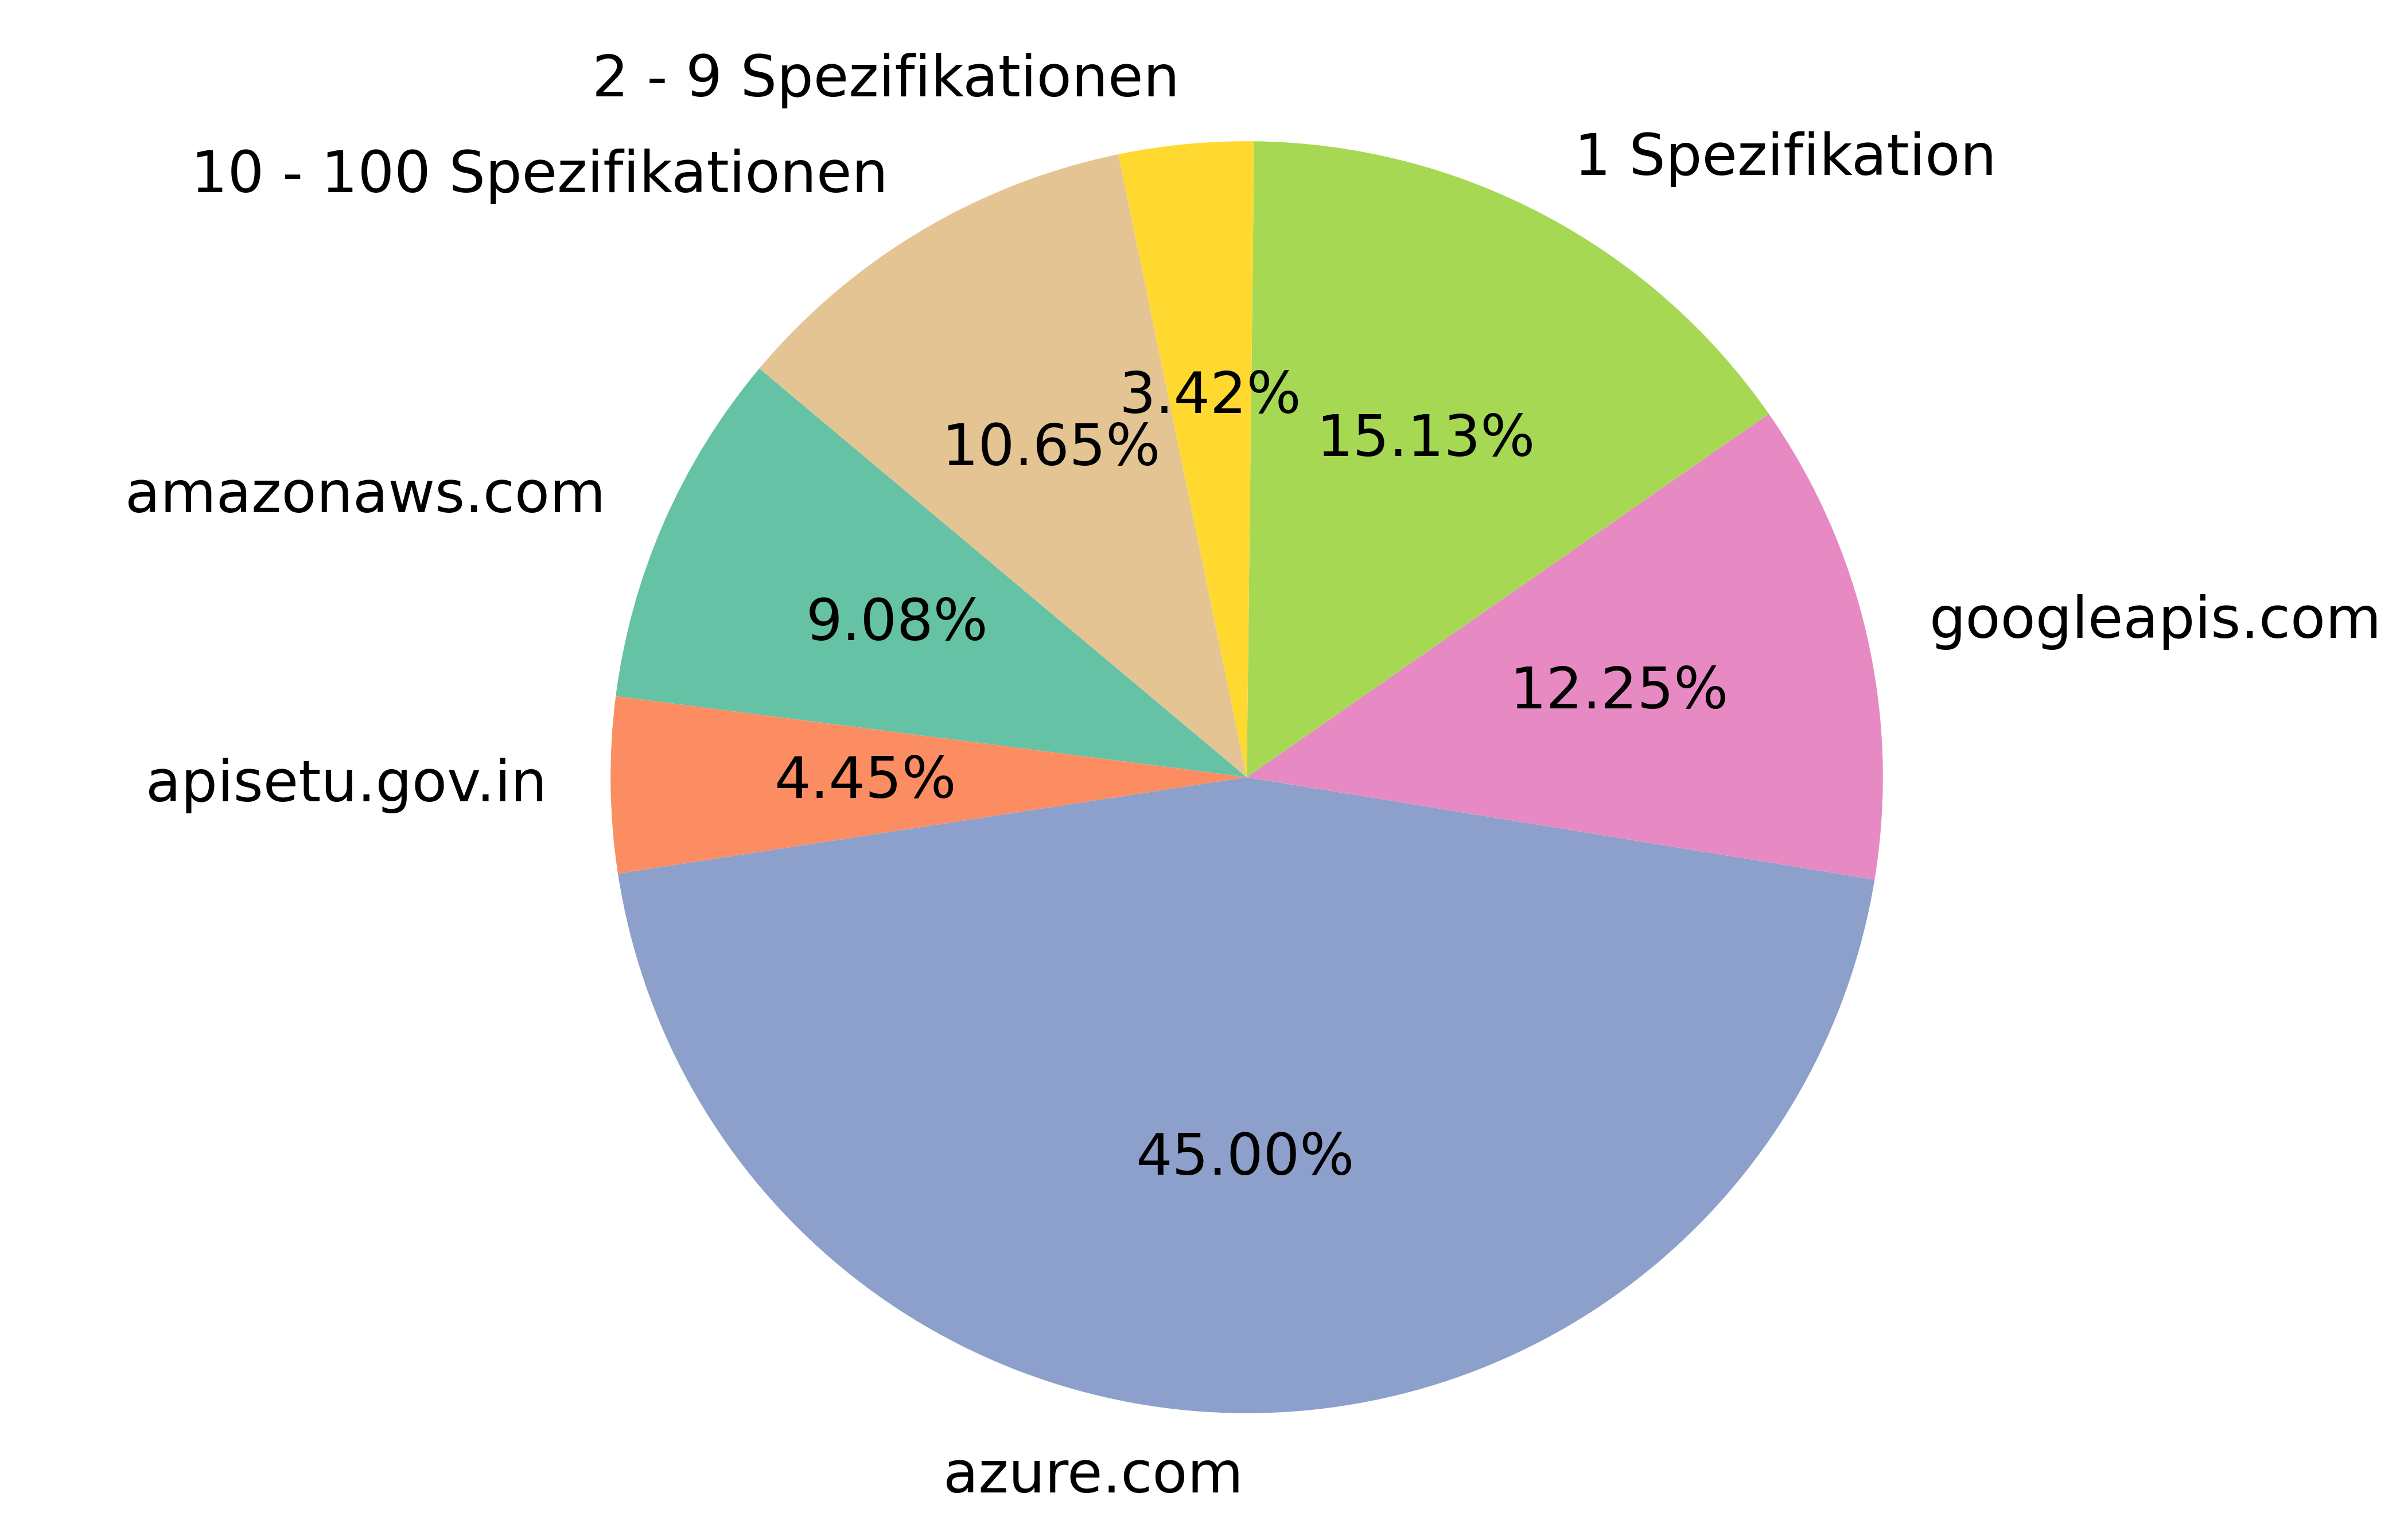
\includegraphics[width=1\textwidth]{img/defense-specificationsperdomainpie.png}
        \caption{Anzahl der Spezifikationen pro Anbieter}
        \label{fig:Specifications}
      \end{figure}    
    \end{column}
    \begin{column}{0.5 \textwidth}
      \begin{figure}[htbp]
        \centering
        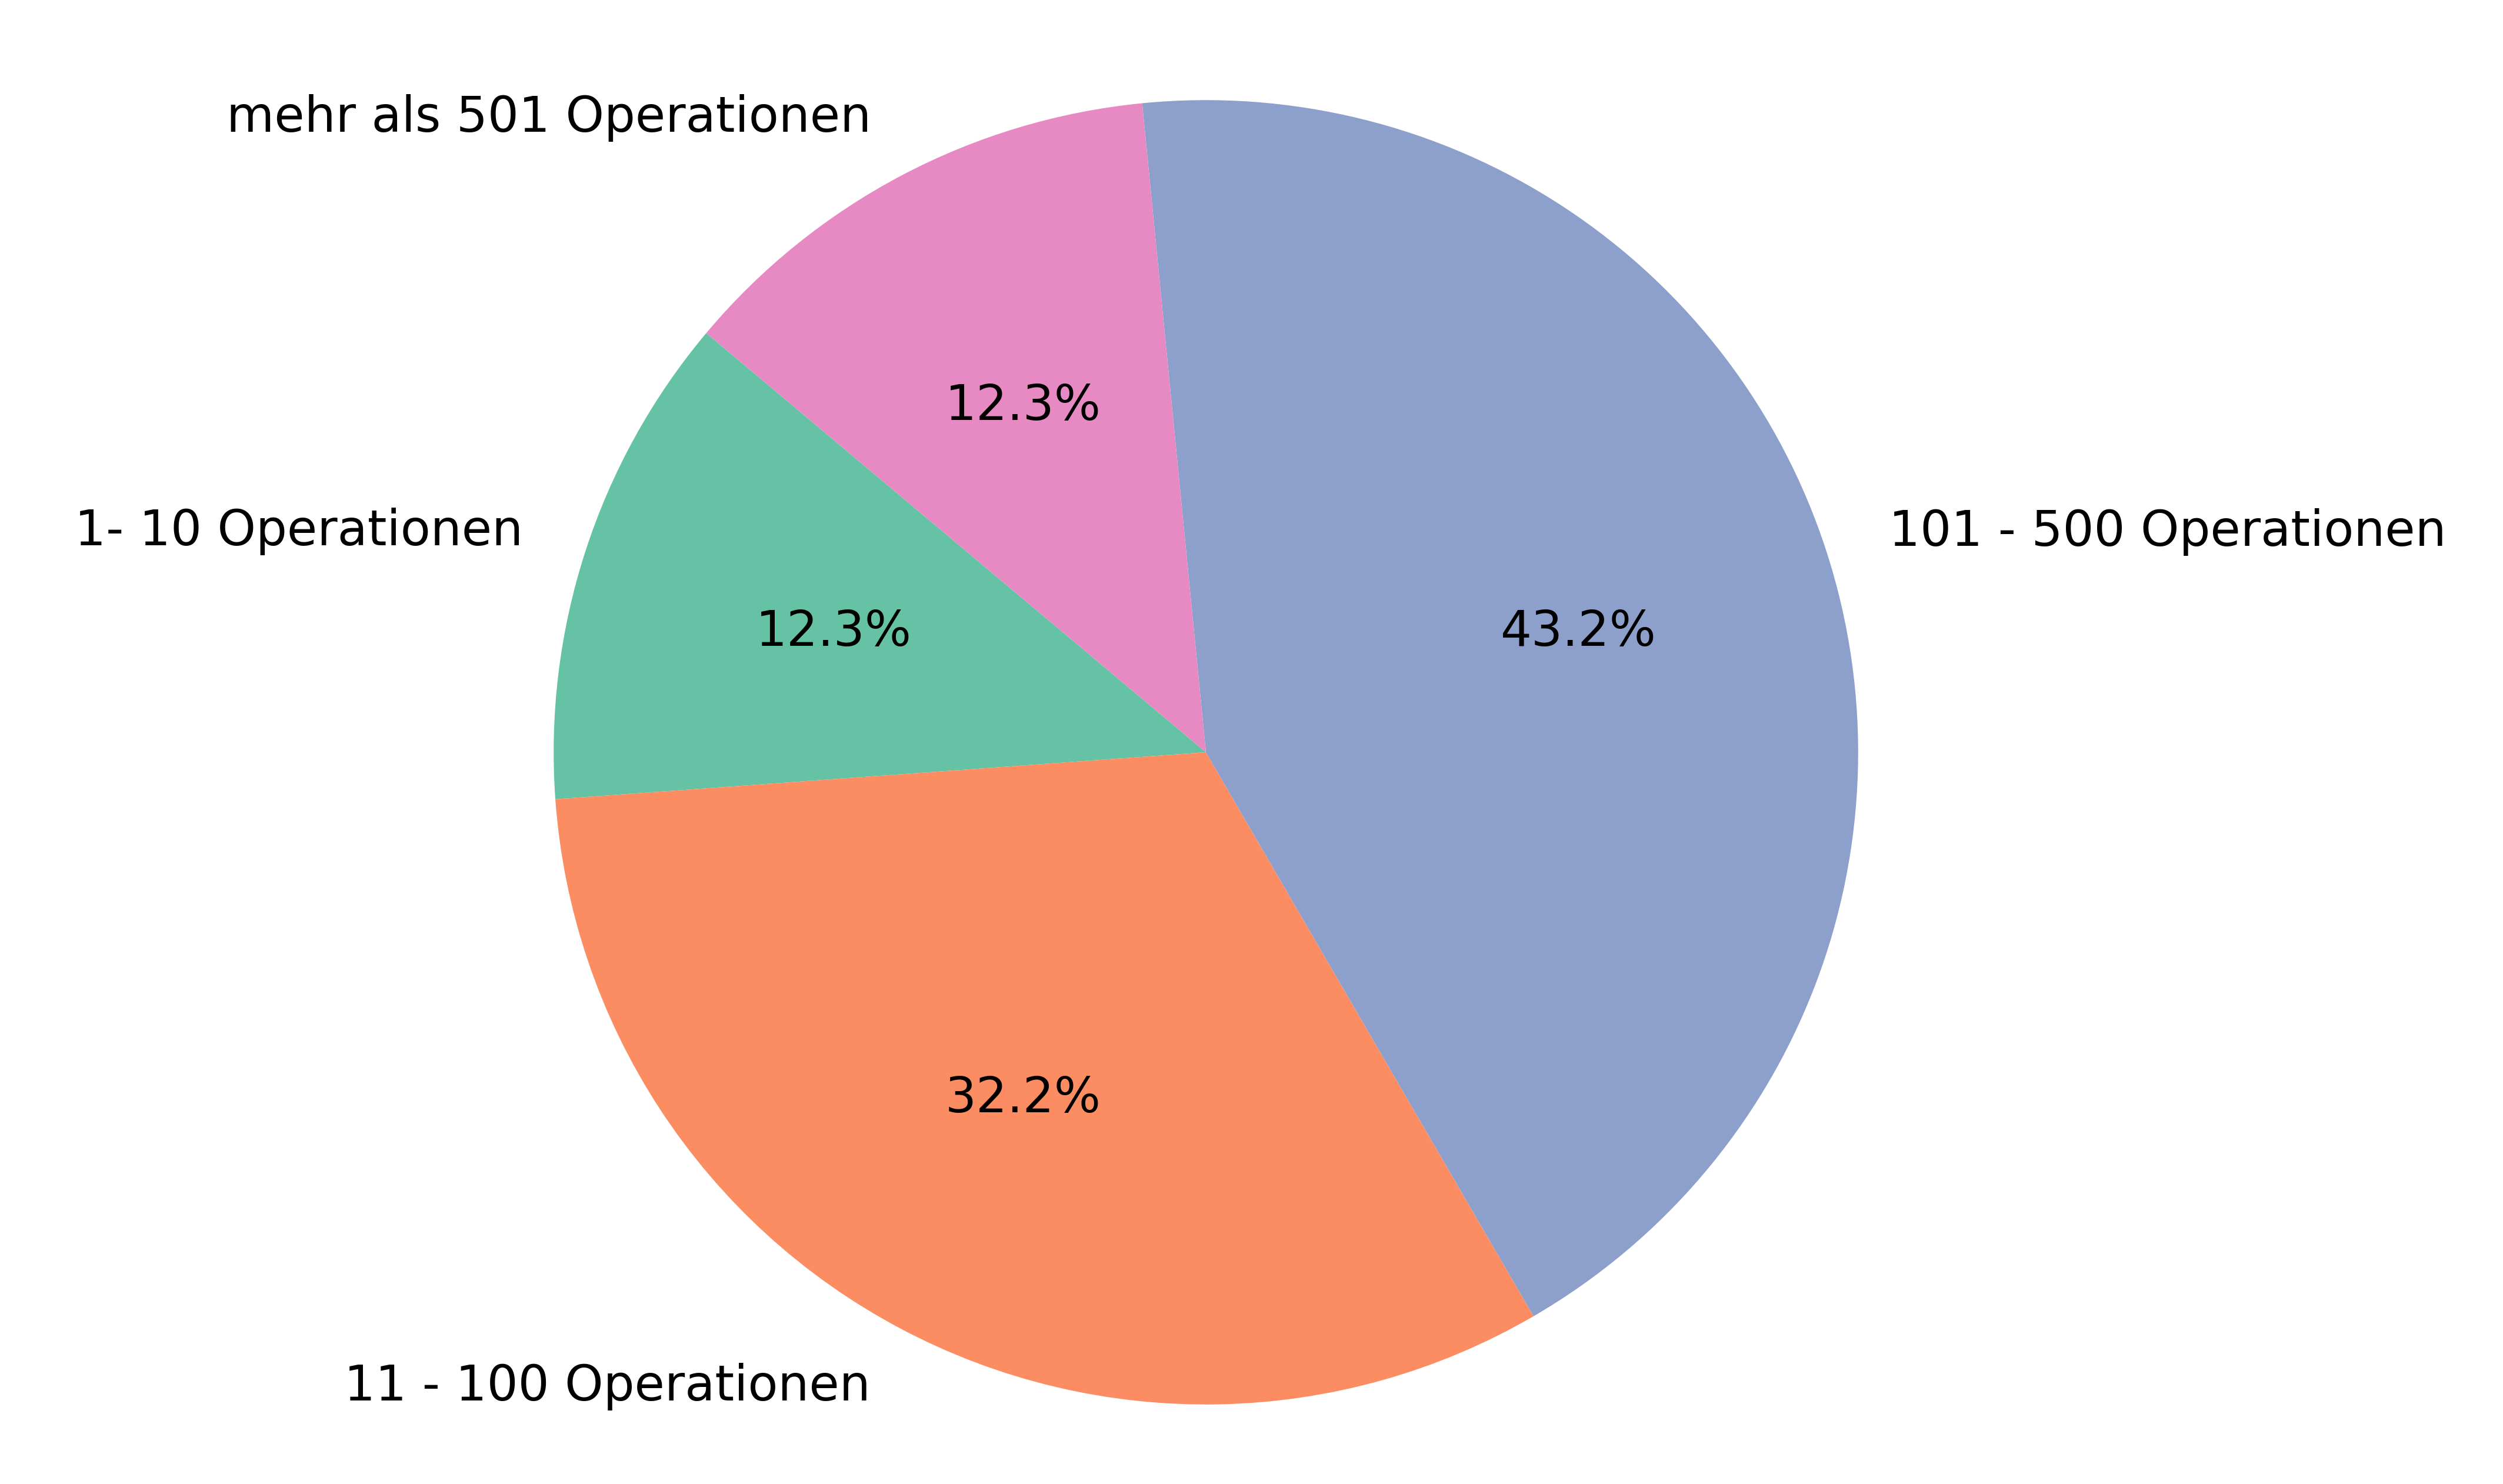
\includegraphics[width=1\textwidth]{img/defense-operationsperspecificationpie.png}
        \caption{Anzahl der API Operationen pro Spezifikation}
        \label{fig:Operations}
      \end{figure}    
    \end{column}
  \end{columns}
\end{frame}

\section{Methodik}
\subsection{Use Cases}
\begin{frame}
  \frametitle{Linting}
  \vspace{-0.5cm}
  \begin{figure}[htbp]
    \centering
    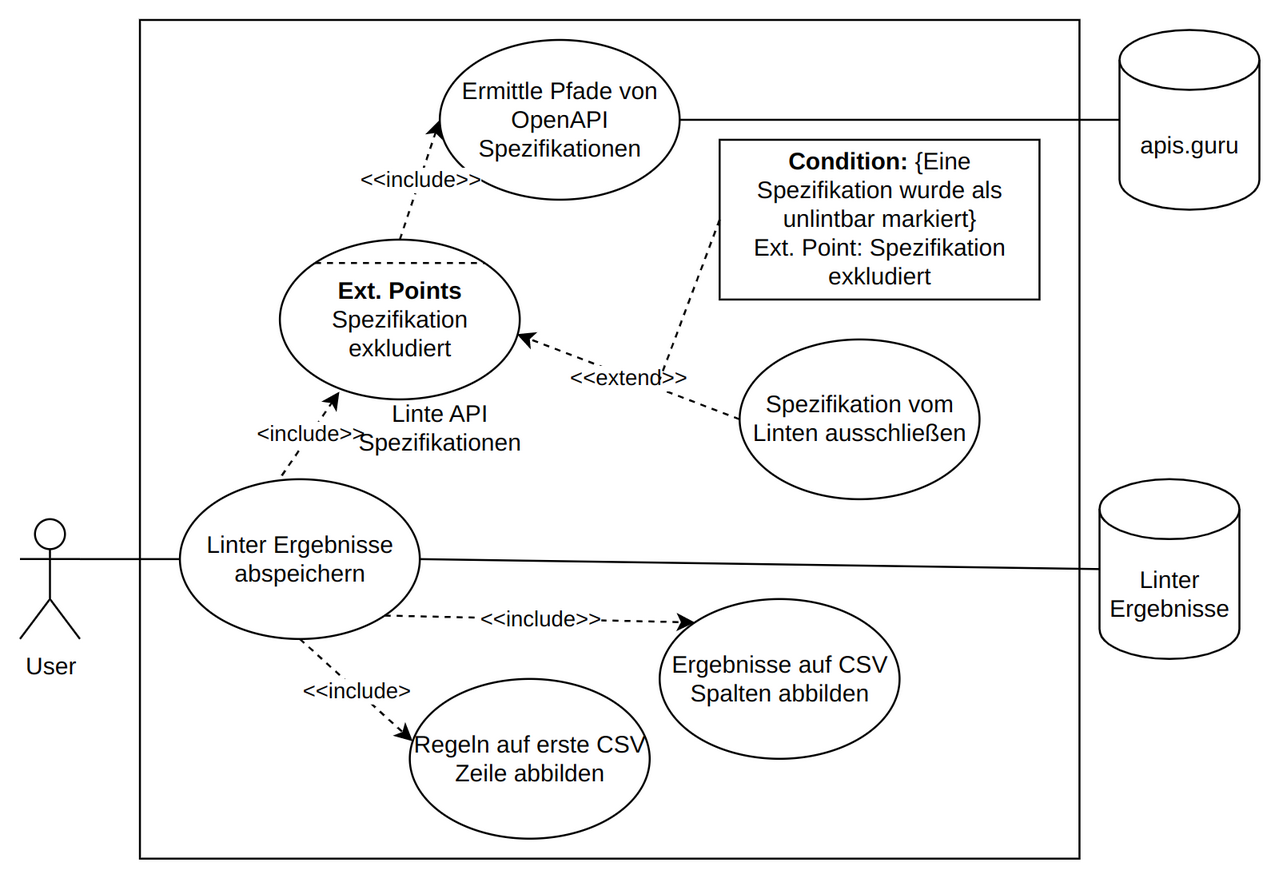
\includegraphics[width=0.9\linewidth]{img/defense-linting.png}
    \caption{\textbf{UC-1} Linting}
    \label{fig:linting}
  \end{figure}
\end{frame}

\begin{frame}
  \frametitle{Invertierung}
  \begin{itemize}
    \item Invertierung der Linterfehler ist definiert als Anteil ausgelöster Linterfehler an möglichen Linterfehlern.
    \item Regelklassen:
    \begin{enumerate}
      \item \textbf{Single Trigger:} Regel kann ein Mal ausgelöst werden.
      \item \textbf{Multi Trigger:} Regel kann mehrfach ausgelöst werden.
      \item \textbf{Multi Message:} Regel kann mehrfach ausgelöst werden. An einer selektierten Stelle können Linterfehler mit unterschiedlichen Fehlermeldungen ausgelöst werden.
    \end{enumerate}
  \end{itemize}
\end{frame}

\subsection{Softwarearchitektur}
\begin{frame}
  \frametitle{Softwarearchitektur}
  \vspace{-0.5cm}
  \begin{figure}[htbp]
    \centering
    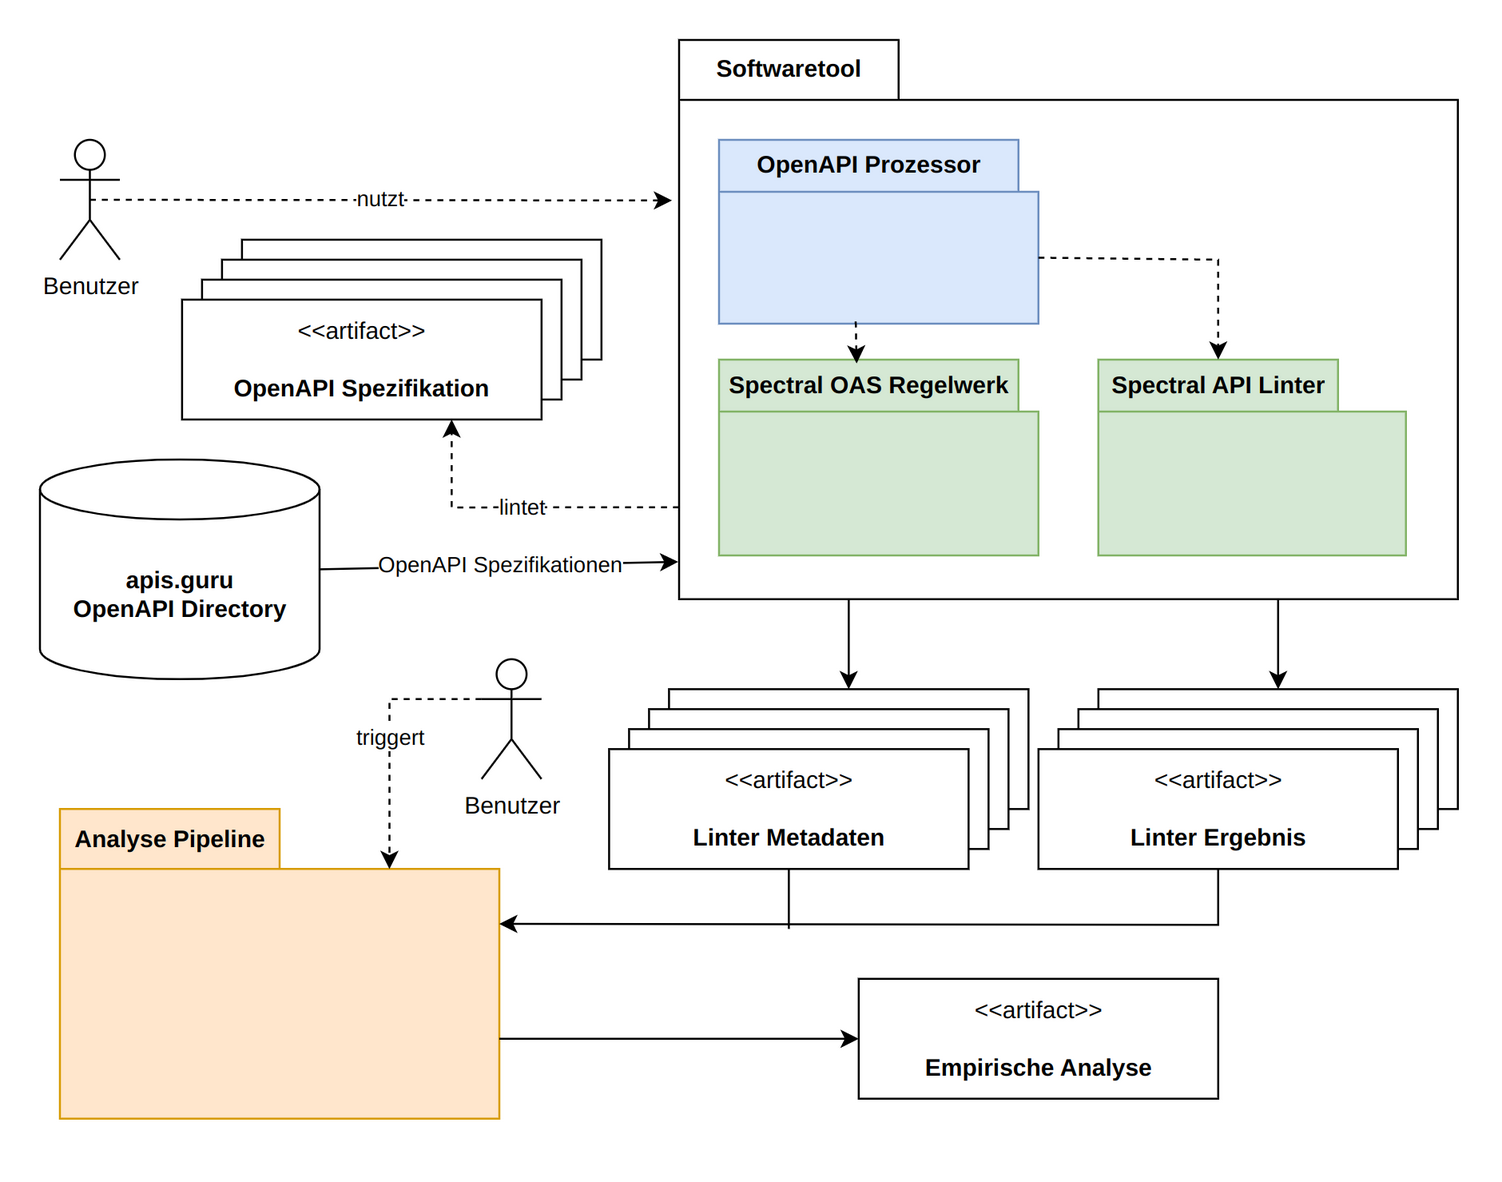
\includegraphics[width=0.8\linewidth]{img/defense-contextview.png}
    \caption{Kontextsicht des Systems}
    \label{fig:Kontextsicht}
  \end{figure}
\end{frame}

\section{Ergebnisse}
\subsection{Explorative Datenanalyse}
\begin{frame}
  \frametitle{Ergebnisse}
  \vspace{-0.4cm}
  \begin{itemize}
    \item 929.699 Linterfehler.
    \item 7.778.972 mögliche Stellen für Linterfehler.
  \end{itemize}
  \begin{figure}[htbp]
    \centering
    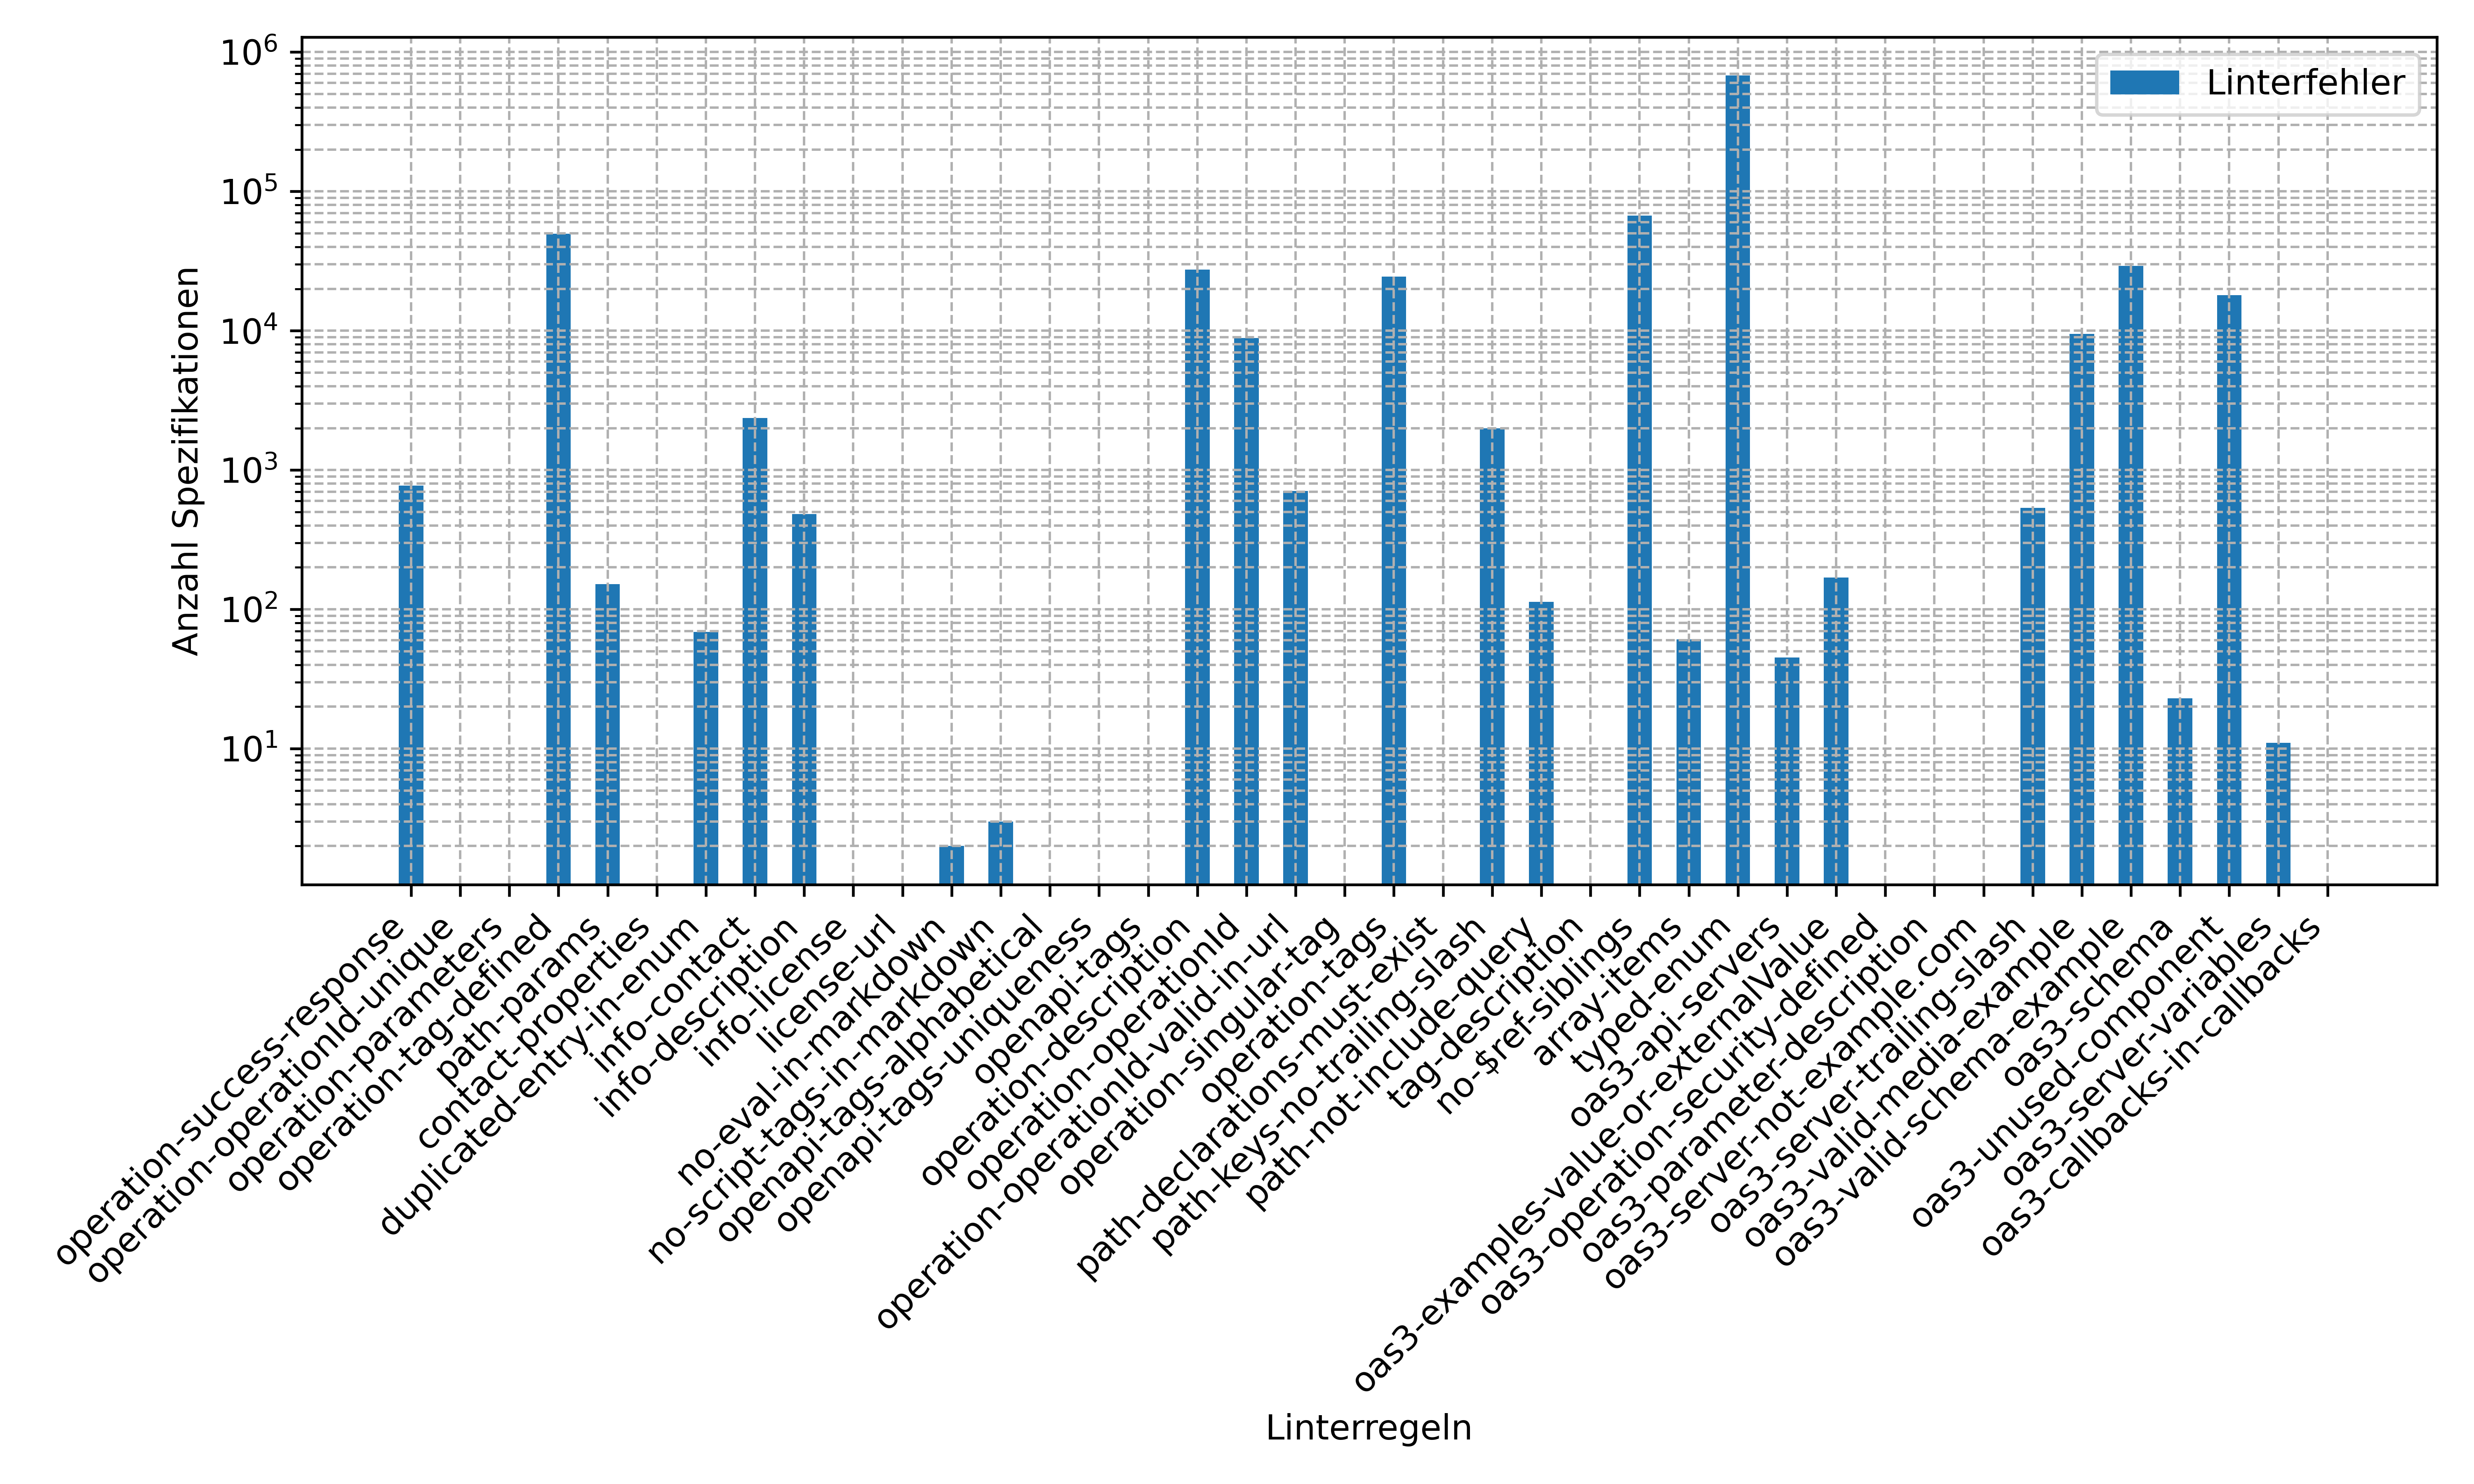
\includegraphics[width=0.9\linewidth]{img/defense-totalspecthrownbarplot.png}
    \caption{Übersicht aller geworfenen Linterfehler}
    \label{fig:totalthrown}
  \end{figure}
\end{frame}

\begin{frame}
  \frametitle{Verzerrung des Datensatzes}
  \begin{itemize}
    \item \textbf{Frage:} Hat die Nutzung des Spectral Linters durch den Anbieter Azure.com einen Einfluss auf die Linterfehler?
    \item \textbf{Methode:} t-Test für unabhängige Stichproben.
    \item \textbf{Ergebnis:} Der durchschnittliche Anteil an Azure.com Linterfehlern ist niedriger, wenn Azure.com die Regel anwendet. 
  \end{itemize}
\end{frame}

\begin{frame}
  \frametitle{Ergebnisse der Invertierung}
  \vspace{-0.4cm}
  \begin{itemize}
    \item Ansatz nur für Single Trigger und Multi Trigger gültig.
    \item Invertierung vielversprechend für genauere Priorisierungen.
  \end{itemize}
  \begin{figure}[htbp]
    \centering
    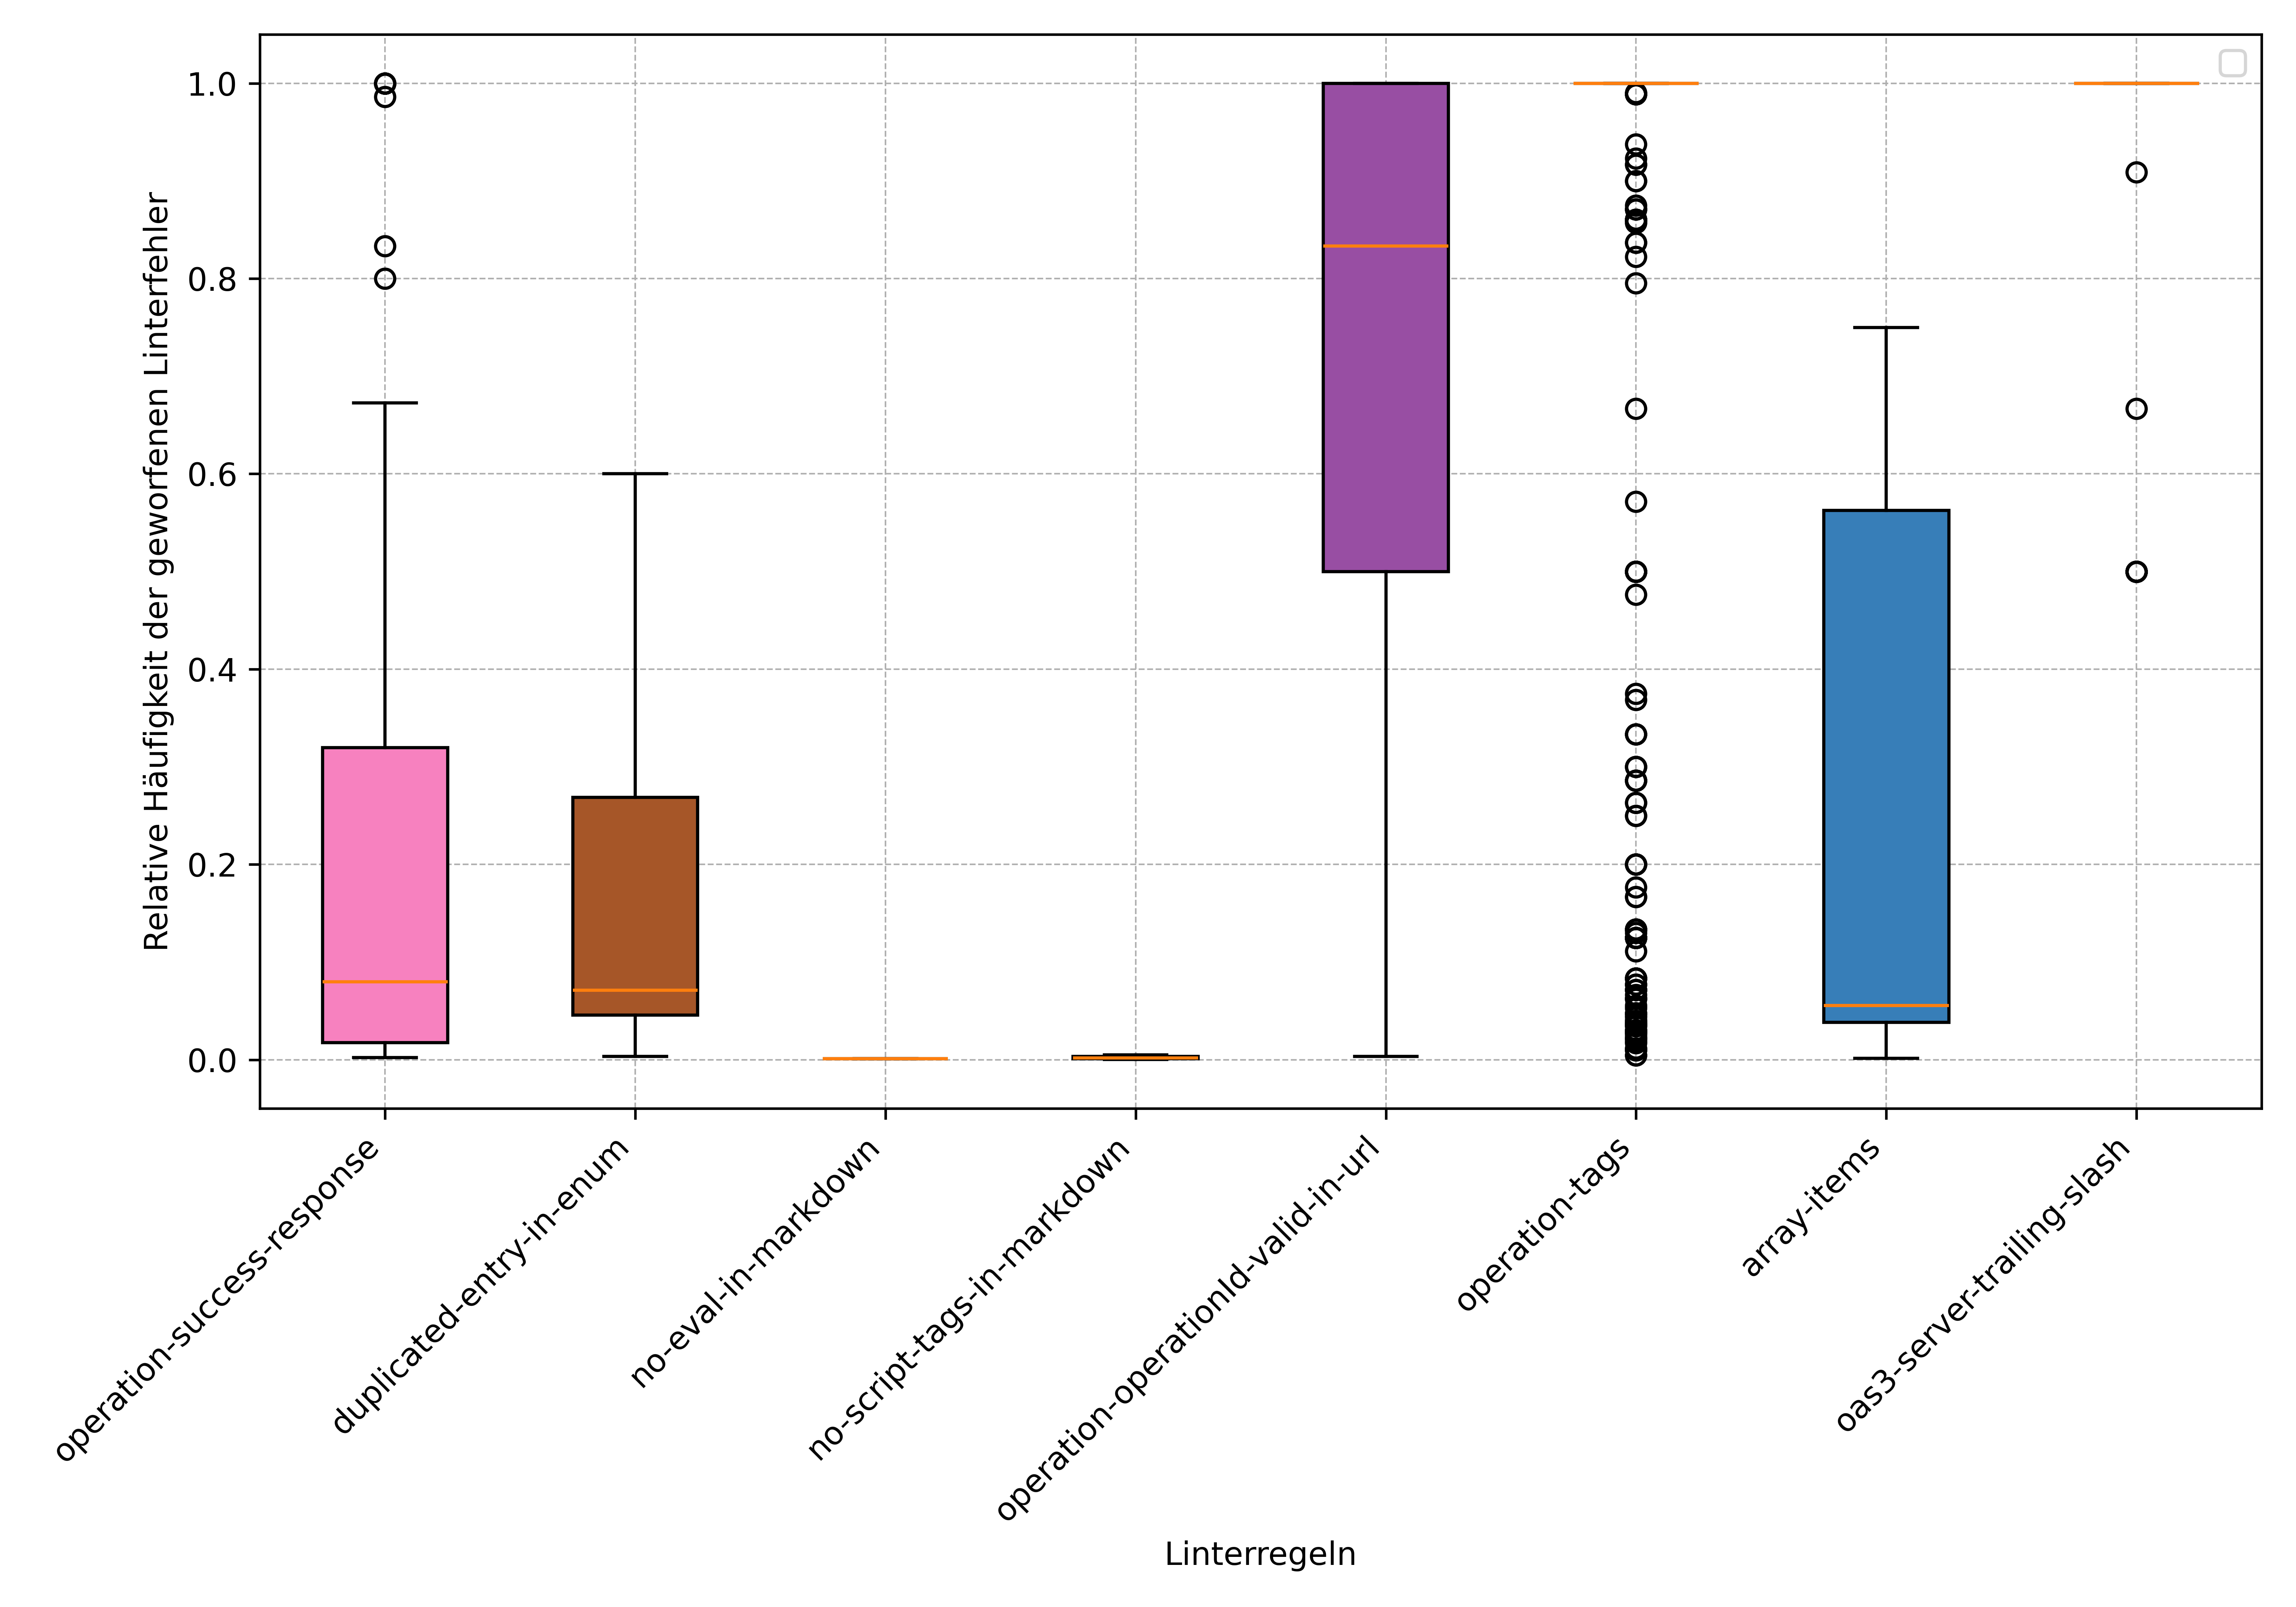
\includegraphics[width=0.75\linewidth]{img/defense-boxplotcleanmultitrigger.png}
    \caption{Multi Trigger Regeln Auslösehäufigkeit}
    \label{fig:boxplot}
  \end{figure}
\end{frame}

\subsection{Priorisierung}
\begin{frame}
  \frametitle{$\text{Relevanz}_\text{Frequenz}$}
  \vspace{-0.4cm}
  \begin{itemize}
    \item Bewertung der Anzahl der Auslösungen einer Regel.
    \item Regeln, die häufig ausgelöst werden, sind weniger relevant.
  \end{itemize}
  \begin{greyblock}{Berechnungsfunktion}
    \scriptsize{
      \[
        \text{Relevanz}_\text{Frequenz}(r) = 
        \begin{cases}
        1&\text{, wenn } 0 =  summe(r)\\
        \frac{1}{summe(r)}&\text{, sonst}.
        \end{cases}
      \]
      \[
        summe(r) = \sum_{i=1, \: i \in S}^{n}vorkommen(r, i)
      \]
      \[
        vorkommen(r, s) = 
        \begin{cases} 
        1&\text{, wenn die Spezifikation } s \text{ die Regel } r \text{ ausgelöst hat}, \\
        0&\text{, sonst}.
        \end{cases}
      \]
      \[
        r \in R, \text{ wobei $R$ die Menge aller OAS Linterregeln ist.}
      \]
      \[
       s \in S, \text{ wobei $S$ die Menge aller Spezifikationen im OpenAPI Directory ist.}
      \]
      \[
        n = \vert S \vert
      \]
    }
  \end{greyblock}
\end{frame}

\begin{frame}
  \frametitle{$\text{Relevanz}_\text{Diversität}$}
  \vspace{-0.6cm}
  \begin{itemize}
    \item Bewertung der Ähnlichkeit des Auslösemusters einer Regel.
    \item Regeln mit einem einzigartigen Auslösemuster sind relevanter.
  \end{itemize}
  \begin{greyblock}{Berechnungsfunktion}
    \scriptsize{
      \[
        \text{Relevanz}_\text{Diversität}(r) = (\frac{1}{n} \sum_{i=1, \: i \in R}^{n} 1- Jaccard(r, r_i))
      \]
      \[
        Jaccard(A,B)=\frac{\vert A \cap B \vert}{\vert A \vert + \vert B \vert - \vert A \cap B \vert}
      \]
      \[
        r \in R, \text{ wobei $R$ die Menge aller OAS Linterregeln ist.}
      \]
      \[
       S \text{ ist die Menge aller Spezifikationen im OpenAPI Directory.}
      \]
      \[
      0 \leq Jaccard(A, B) \leq 1, \quad A, B \in \mathbb{B}^m, \quad n = \vert R \vert, \quad m = \vert S \vert
      \]
    }
  \end{greyblock}
\end{frame}  

\begin{frame}
  \frametitle{Relevanz}
  \vspace{-0.4cm}
  \begin{itemize}
    \item Beide Verfahren teilen Regeln in zwei Gruppen.
    \item Regeln, die nie ausgelöst  werden, sind am relevantesten.
  \end{itemize}
  \begin{figure}[htbp]
    \centering
    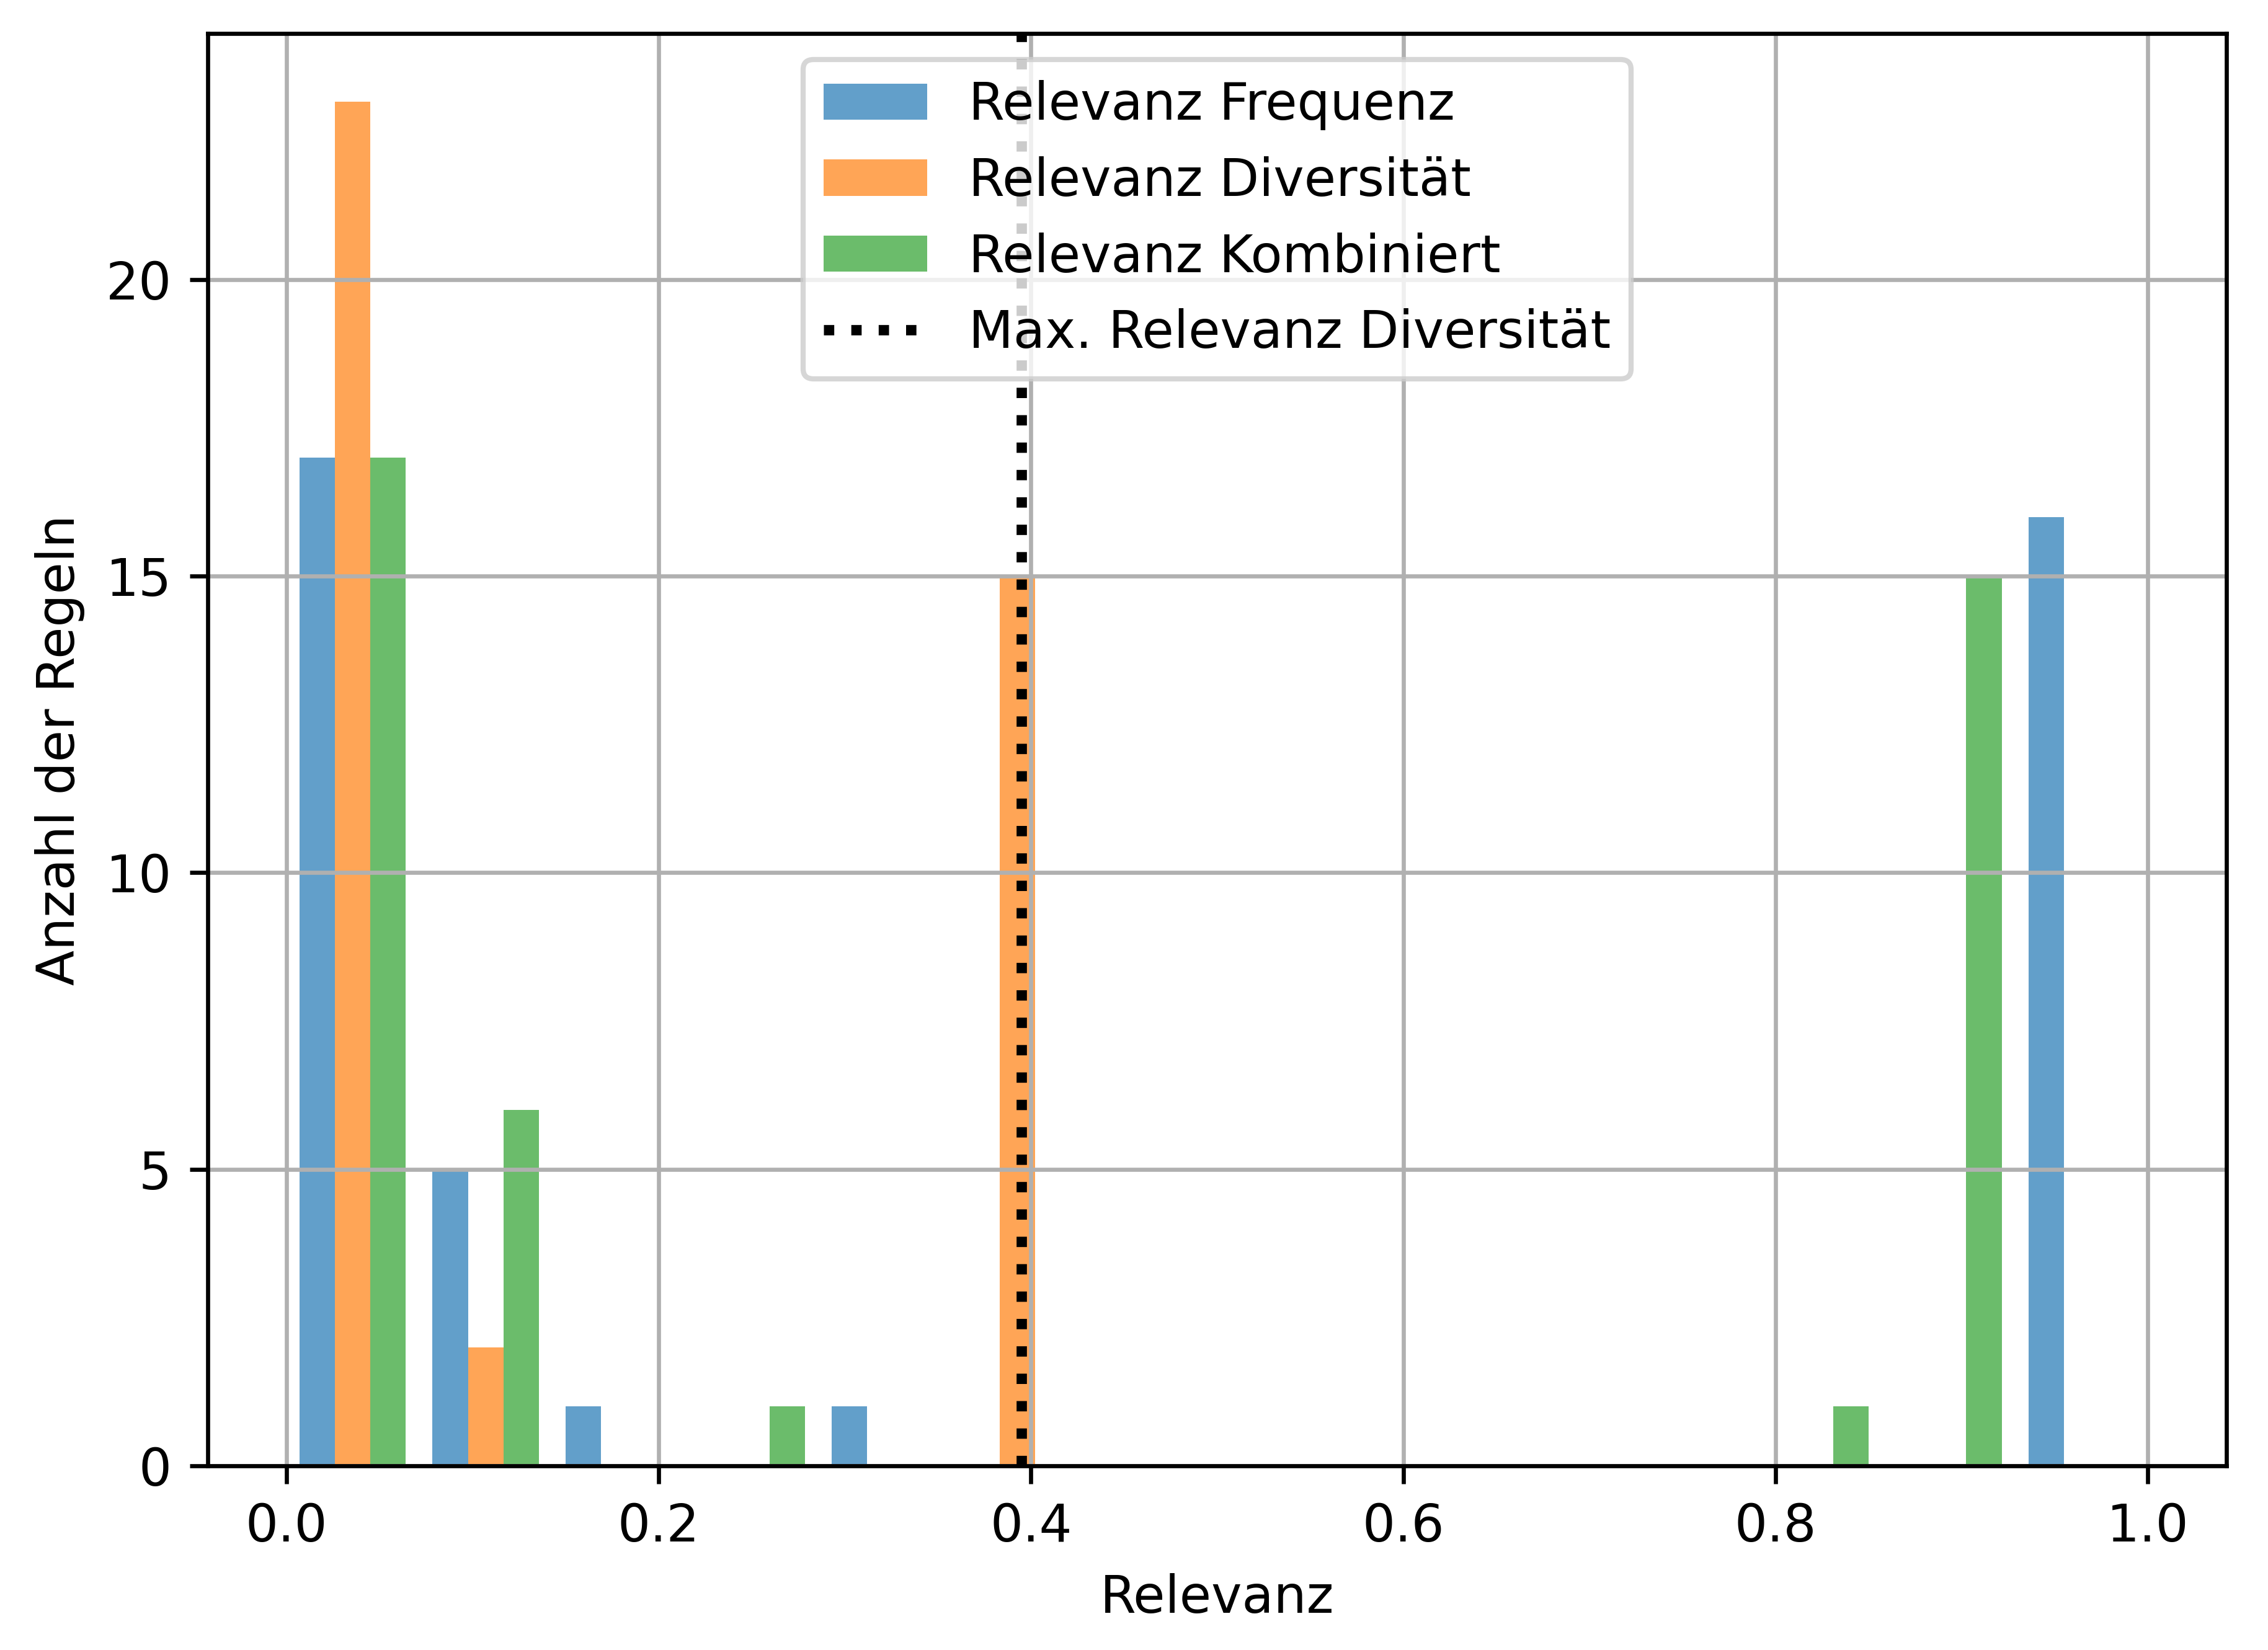
\includegraphics[width=0.72\linewidth]{img/defense-priodistrhist.png}
    \caption{Relevanz der Regeln}
    \label{fig:histogram}
  \end{figure}
\end{frame}

\subsection{Neuzuordnung der Schweregrade}
\begin{frame}
  \frametitle{Clustering}
  \vspace{-0.4cm}
  \begin{itemize}
    \item Neuzuordnung der Schweregrade mit k-means Clustering.
  \end{itemize}
  \begin{figure}[htbp]
    \centering
    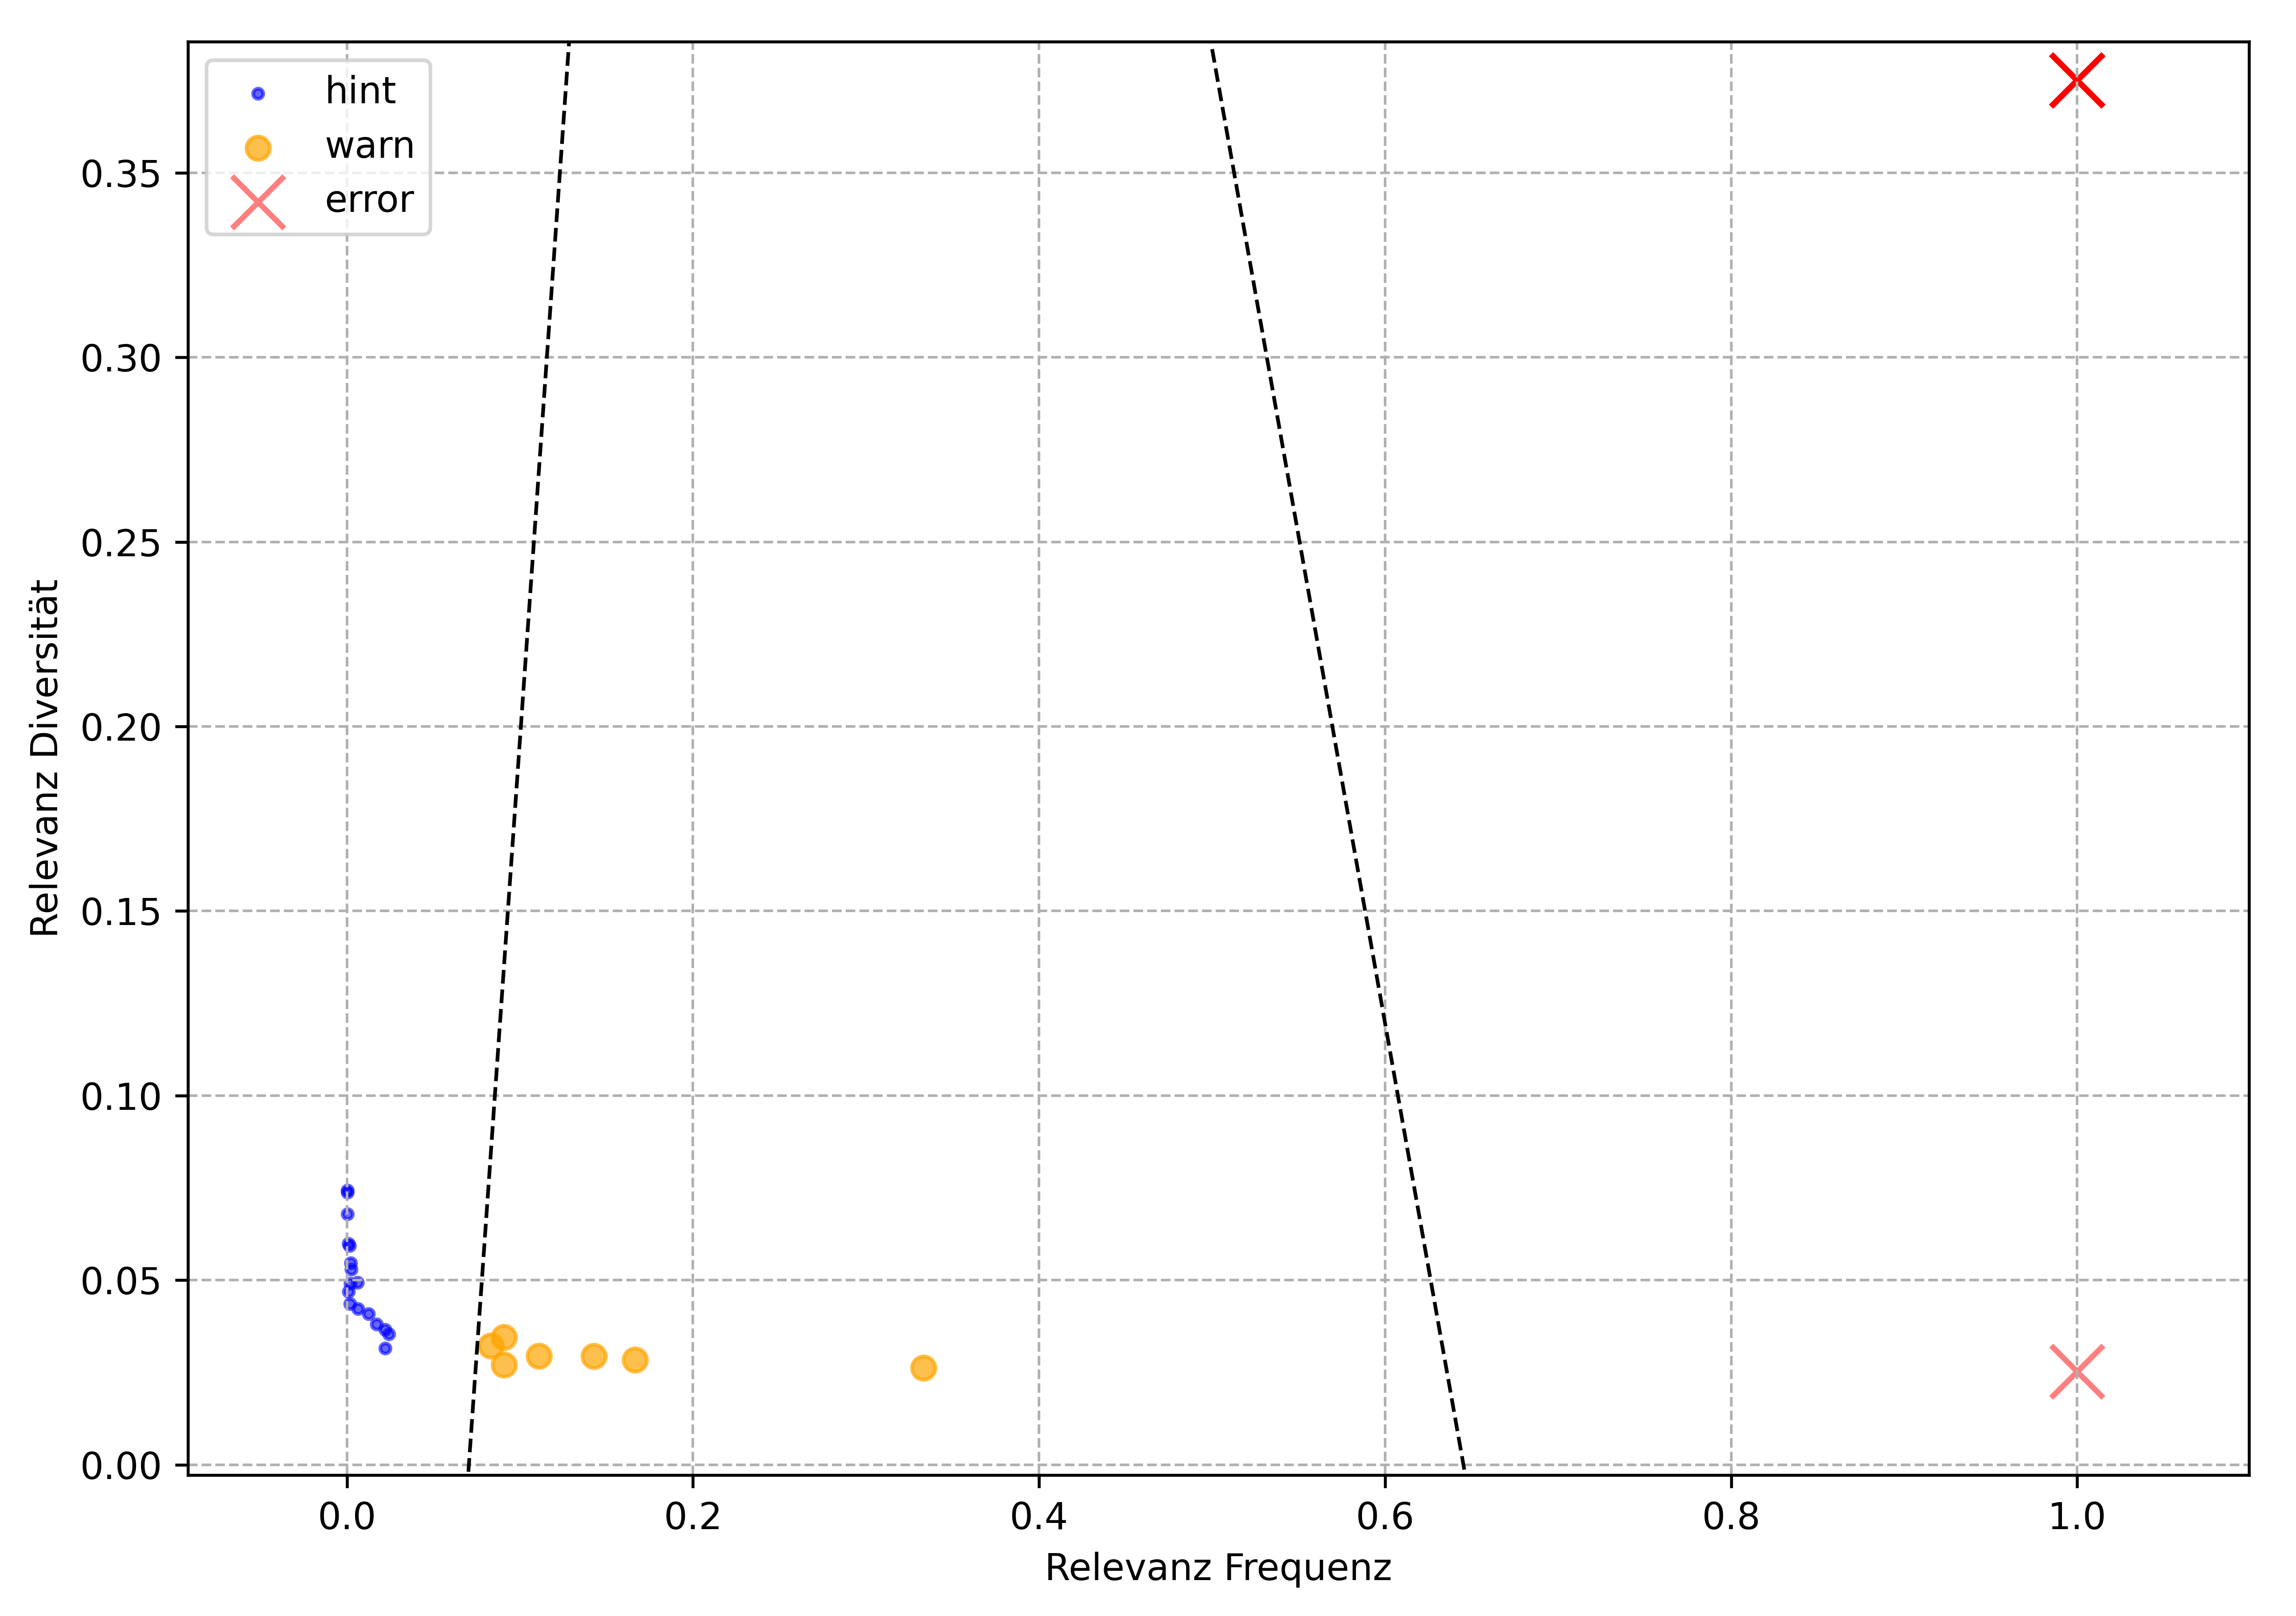
\includegraphics[width=0.82\linewidth]{img/defense-clusterprioscatter.png}
    \caption{Neuzuordnung mit Clustering}
    \label{fig:clustering}
  \end{figure}
\end{frame}

\begin{frame}
  \frametitle{Umverteilung der Schweregrade}
  \begin{longtable}{llr}
    \label{tab:severityreassignments}
    \endfirsthead
    \endhead
    \textbf{Schweregrad OAS} & \textbf{Schweregrad Cluster} & \textbf{Anzahl} \\ \hline
    \textcolor{blue}{\texttt{hint}} & \textcolor{blue}{\texttt{hint}} & 4 \\
    \textcolor{orange}{\texttt{warn}} & \textcolor{orange}{\texttt{warn}} & 4 \\
    \textcolor{red}{\texttt{error}} & \textcolor{red}{\texttt{error}} & 1 \\
    \textcolor{orange}{\texttt{warn}} & \textcolor{red}{\texttt{error}} & 13 \\
    \textcolor{orange}{\texttt{warn}} & \textcolor{blue}{\texttt{hint}} & 12 \\
    \textcolor{blue}{\texttt{hint}} & \textcolor{orange}{\texttt{warn}} & 3 \\
    \textcolor{blue}{\texttt{hint}} & \textcolor{red}{\texttt{error}} & 1 \\
  \caption{Neuverteilungen der Linter Schweregrade}
  \end{longtable}
\end{frame}

\subsection{Ergebnisdemonstration}
\begin{frame}
  \centering{\textbf{Ergebnisdemonstration}}
\end{frame}

\section{Fazit}
\begin{frame}
  \frametitle{Fazit}
  \begin{itemize}
    \item Potenzial von Invertierungen konnte in Priorisierung der Regeln nicht ausgeschöpft werden.
    \item Priorisierungen für die Linterregeln können dazu beitragen, die Ziele zu erreichen.
    \item Subjektive Einschätzungen der Relevanz von Linterregeln sind wichtig und lassen sich durch die Methode nicht ersetzen.
  \end{itemize}
\end{frame}